\chapter{Observace, měření a reprezentace}
K pozorování meteorů a jejich záznamu se v současnosti používají tři přístupy: fotografické snímky, videozáznamy a radarová měření.

Ve všech třech přístupech je cílem sledovat a zaznamenávat celou oblohu nebo alespoň její velkou část. Například u fotografického přístupu se používá rybí oko \cite{ceplecha} -- čočka nebo objektiv, který je schopný zobrazit celou oblohu na jeden snímek. Cenou za takto širokoúhlý snímek je velké zkreslení obrazu, to lze ale pro účely měření matematicky odstranit \cite{ceplecha}.

\todo{Radarová měření dle \cite{radiosurvey}}

Fotografické snímky a videozáznamy jsou z hlediska měření velmi blízké: Videozáznam je v principu pouze série fotografií, v minulém století se ale využívalo spíše opačného přístupu, kdy se několik fotografických záběrů zaznamenalo na jeden snímek \cite{ceplecha}. Oba přístupy tedy dávají průběh polohy (a případně i luminosity) meteoru v čase. Konkrétně pro metody identifikace meteorických rojů potřebujeme právě dráhu (polohu) a rychlost meteoru \cite{ceplecha}, abychom zjistili orbitální dráhu meteoroidu. Důkladněji se zpracování fotografických snímků budeme věnovat v sekci \ref{sec:foto}.

\section{Elementy dráhy}
Orbitální dráhy jsou v prvním přiblížení elipsy, které jsou nakloněné v prostoru. Jedním z ohniskových bodů je vždy těžiště (Sluneční) soustavy, pro určení dráhy tedy stačí 5 parametrů \cite{astro}.

\smallskip

Dva z parametrů popisují tvar elispy; její velikost a excentricitu \cite{astro}. \textit{Excentricita} $e$ náleží do intervalu $\left[0,1\right)$,\footnote{Excentricita může být také $=1$ pro parabolické a $>1$ pro hyperbolické dráhy. \ask{Otevřené, předpokládám, ignorujeme, protože by patřily do sporadického pozadí automaticky (nemají mateřský objekt ve Sluneční soustavě).}} a udává, jak blízká kružnici tato dráha je (viz obrázek \ref{img:excentricity}).

\todo{Ilustrace excentricit}

Pro určení velikosti používáme buďto \textit{délku hlavní poloosy} $a$ nebo \textit{vzdálenost perihelia} $q$ (efektivně vzdálenost okraje elipsy od ohniska). Jejich vztah ilustruje obrázek \ref{img:elipsa} a mezi oběma lze převádět pomocí rovnice \cite{ceplecha}
$$
    q=a(1-e)\text{.}
$$

\todo{Obrázek vztahu mezi $a$ a $q$}

\smallskip

Zbylé tři parametry určují natočení elipsy v prostoru. Jedná se o obdobu Eulerových úhlů, jsou ovšem definované vůči Slunci a ekliptice. Tyto úhly jsou znázorněny v obrázku \ref{img:elementy} a slovně se jedná o
\begin{itemize}
    \item \textit{inklinaci} $i$, která udává úhel mezi rovinou ekliptiky a rovinou elipsy \cite{astro},
    \item \textit{délku vzestupného uzlu} $\Omega$, která udává heliocentrickou ekliptikální délku bodu, ve kterém dráha protíná rovinu ekliptiky při průletu z jihu (tzv. \textit{vzestupný uzel}, \NorthNode) \cite{astro}, a
    \item \textit{argument perihelia} $\omega$, úhel, ve kterém se nachází perihelium, měřený od úsečky spojující Slunce a vzestupný uzel \cite{astro}.
\end{itemize}
Tyto úhly se aplikují jako rotace na rovinu ekliptiky s počátkem ve středu Slunce.

\begin{figure}[ht]
    \centering
    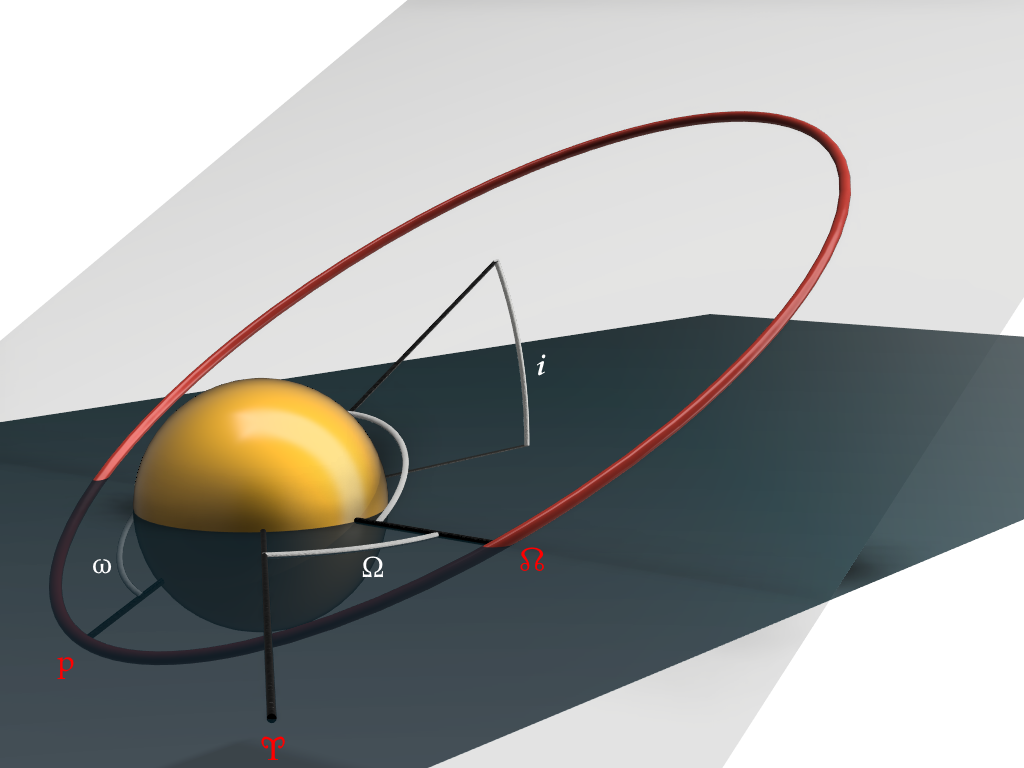
\includegraphics[width=0.8\linewidth]{img/orbit-elements-marked.png}
    \caption{Ilustrace významu elementů dráhy $i$, $\Omega$ a $\omega$ \cite{astro}}
    \label{img:elementy}
\end{figure}

\smallskip

Na takto definované dráze se ještě můžeme setkat se souřadnicí zvanou \textit{pravá anomálie} $\nu$. Ta již nespecifikuje dráhu, nýbrž polohu objektu na své dráze, a v meteodách identifikace meteorických rojů nevystupuje. Udává se jako úhel měřený od spojnice Slunce a perihelia ke spojnici Slunce a objektu \cite{astro}.

\section{Fotografická měření\label{sec:foto}}
Úkolem astrometrických měření meteorů je zjistit elementy dráhy meteoroidu před tím, než se setkal s atmosférou Země. Vše ale začíná na fotografii nebo videozáznamu průletu meteoru atmosférou.

Budeme popisovat techniku měření používanou pro fotografická měření, kde máme fotoaparát s rybím okem pro zachycení celé oblohy a clonou, která s pevnou periodou (několikrát za vteřinu) zakrývá detektor nebo fotografický film, čímž zachytí časovou závislost pohybu meteoru. \todo{Bude-li obrázek, přidat a popsat.} Pro video je postup prakticky identický, hůře se ale ilustruje.

\smallskip

Mějme tedy stanici \textbf{A} ležící na zeměpisné šířce $\varphi_\mathbf{A}$ a zeměpisné délce $\lambda_\mathbf{A}$, kde je umístěn fotoaparát s rybím okem a periodickou clonou tak, že zenit (kolmice k zemskému geoidu) leží uprostřed snímku, a přesné hodiny pro zaznamenání času měření. Fotoaparát v průběhu noci pořídí velké množství snímků a ke každému snímku umíme přiřadit přesný čas.

Prvním krokem při zachycení meteoru je získat z fotografie jeho polohu v obrozníkové soustavě.

Začneme zavedením kartézských souřadnic na snímku s počátkem ve středu fotografie, který by měl být polohou zenitu. Pro každý otisk meteoru na snímku naměříme souřadnice $x_i,y_i$ v arbitrárních jednotkách a stejně tak na snímku naměříme souřadnice hvězd. Jelikož polohy hvězd jsou velmi přesně měřeny a katalogovány, ke každé hvězdě dopočteme také azimut a zenitovou vzdálenost z katalogových údajů a \todo{Metoda nejmenších čtverců...}